%%%%%%%%%%%%% Doing my own template
%%%%%%%%%%%%% Following the specifications of
% http://bu.univ-amu.libguides.com/c.php?g=511743&p=4025195
%%%%%%%%%%%%% Sober amu thesis template

% LAYOUT %%%%%%%%%%%%%%%%%%%%%%%%%%%%%%%%%%%%%%%%%%%%
%%% Using the report class
\documentclass[12pt, 			% Recommended
               singlespacing,         % SHOULD BE
               %singlespacing
			  ]{report}

%%% Margins
\usepackage[a4paper,
			%width=150mm,
			top=30mm,
			bottom=30mm,
            right=30mm,
            left=30mm,
            % Offset to bind pages
            bindingoffset=6mm,  
            % To make room for the header
            headheight=20mm,    
           ]{geometry}

% Line spacing - 1 is normal, 1.3 is onehalf and 1.6 is double spacing
\linespread{1}

%%% Change titles & stuff
\makeatletter
\renewcommand{\@chapapp}{Section}
\makeatother
\renewcommand{\abstractname}{Résumé}
\renewcommand{\contentsname}{Table des matières}
\renewcommand{\appendixname}{Table des annexes}

%%%%%%%%%%%%%%%%%%%%%%%%%%%%%%%%%%%%%%%%%%%%%%%%%%%%%

% Miscellaneous packages %%%%%%%%%%%%%%%%%%%%%%%%%%%%

%%% Really basic packages here to handle languages
\usepackage[english, french]{babel}
\usepackage[utf8]{inputenc}
\usepackage[T1]{fontenc}
% The font
\usepackage{concmath}
% Highlight stuff for revisions + colors and units
\usepackage{color}
\usepackage[x11names]{xcolor}
\usepackage{graphicx}
\usepackage{amsmath,amssymb, bm}
\usepackage[squaren, Gray, cdot]{SIunits}

\usepackage{listings}

% Where your pictures are
\graphicspath{ {pics/} }

%%% Header & Footer
\usepackage{fancyhdr}
\pagestyle{fancy}
\fancyhead{}
\fancyhead[RO,LE]{\rightmark}
\fancyfoot{}
\fancyfoot[LE,RO]{\thepage}
\fancyfoot[CE,CO]{\leftmark}
\fancyfoot[RE,LO]{}
\renewcommand{\headrulewidth}{0.4pt}
\renewcommand{\footrulewidth}{0.4pt}

% Some symbols
\usepackage{textcomp}

% To include pdfs, like articles, directly
\usepackage{pdfpages}            

% For figures
\usepackage{caption}
\usepackage{subcaption}

% For text boxes spanning multiple pages
% And to add a color to it
\usepackage{framed}
% Access the different colors here
% http://mirrors.standaloneinstaller.com/ctan/macros/latex/contrib/xcolor/xcolor.pdf page 40
\colorlet{shadecolor}{LightSteelBlue1}
\colorlet{framecolor}{Blue4}

% New environment for shaded frames
\newenvironment{frshaded}{%
\def\FrameCommand{
\fboxrule=\FrameRule
\fboxsep=\FrameSep
\fcolorbox{framecolor}{shadecolor}
}%
\MakeFramed {\FrameRestore}}%
{\endMakeFramed}
% Use like this
%\begin{frshaded}
%\end{frshaded}

% To make todo notes, exemple in the intro
\usepackage[textwidth=3cm]{todonotes}

% For appendices
\usepackage[toc,page]{appendix}
% And change the names
\renewcommand{\appendixname}{Annexe}
\renewcommand{\appendixtocname}{Annexes}
\renewcommand{\appendixpagename}{Annexes}

% Line breaks in text
% Warning: should find something better for urls >.<
\sloppy

% Add quotes
\usepackage{dirtytalk}

% Fancy tables
\usepackage{multirow}

% Urls
\usepackage{url}

% for pdf docs to read on computers
% use this when compiling the pdf version (to send by mail)
% comment it when you want to print it
\usepackage{hyperref}

% Package only for the template
\usepackage{lipsum}

%%%%%%%%%%%%%%%%%%%%%%%%%%%%%%%%%%%%%%%%%%%%%%%%%%%%%

% Glossary %%%%%%%%%%%%%%%%%%%%%%%%%%%%%%%%%%%%%%

% if you need a glossary
% \usepackage{glossaries}         
% \makeglossaries

% \newglossaryentry{ABF}{name=ABF, description={Adaptive Biasing Force}}

% Use \newglossaryentry{utc}{name=UTC, description={Coordinated Universal Time}} to add a glossary entry within the document
% Use gls{utc} to use that entry somewhere

%%%%%%%%%%%%%%%%%%%%%%%%%%%%%%%%%%%%%%%%%%%%%%%%%%%%%

% Bibliography %%%%%%%%%%%%%%%%%%%%%%%%%%%%%%%%%%%%%%

% Required to generate language-dependent quotes in the bibliography
\usepackage[autostyle=true]{csquotes}

% Use biber - way better than bibtex
\usepackage[backend=biber,
% 			citestyle=numeric-comp,
%             bibstyle=numeric,
            citestyle=authoryear,
            bibstyle=authoryear,
            %dashed=false,
            sorting=nyt,
            natbib=true,
            doi=true,
            url=false,
            isbn=false,
            eprint=false,
            giveninits=true,
            uniquename=init,
            maxcitenames=1, 
            minbibnames=6, 
            maxbibnames=6
            ]{biblatex}

% The filename of the bibliography
\addbibresource{all.bib} 
% To escape some underscores in the .bib exported from mendeley
\DeclareSourcemap{ % Used when .bib/Bibliography is compiled, not when document is
    \maps{
        \map{ % Replaces '{\_}', '{_}' or '\_' with just '_'
            \step[fieldsource=url,
                  match=\regexp{\{\\\_\}|\{\_\}|\\\_},
                  replace=\regexp{\_}]
        }
        \map{ % Replaces '{'$\sim$'}', '$\sim$' or '{~}' with just '~'
            \step[fieldsource=url,
                  match=\regexp{\{\$\\sim\$\}|\{\~\}|\$\\sim\$},
                  replace=\regexp{\~}]
        }
        \map{ % Replaces '{\_}', '{_}' or '\_' with just '_'
            \step[fieldsource=doi,
                  match=\regexp{\{\\\_\}|\{\_\}|\\\_},
                  replace=\regexp{\_}]
        }
        \map{ % Replaces '{'$\sim$'}', '$\sim$' or '{~}' with just '~'
            \step[fieldsource=doi,
                  match=\regexp{\{\$\\sim\$\}|\{\~\}|\$\\sim\$},
                  replace=\regexp{\~}]
        }
    }
}

% Start with roman numbers until the introduction
\pagenumbering{roman}

% handle the abbverviations ?
% Basic abbreviation page here, you can play around with the two "5cm"
% To increase or decrease the spacing between the abbreviation and the words
\usepackage{calc}
\makeatletter
\newcommand{\tocfill}{\cleaders\hbox{$\m@th \mkern\@dotsep mu . \mkern\@dotsep mu$}\hfill}
\makeatother
\newcommand{\abbrlabel}[1]{\makebox[5cm][l]{\textbf{#1}\ \tocfill}}
\newenvironment{abbreviations}{\begin{list}{}{\renewcommand{\makelabel}{\abbrlabel}%
        \setlength{\labelwidth}{5cm}\setlength{\leftmargin}{\labelwidth+\labelsep}%
                                              \setlength{\itemsep}{0pt}}}{\end{list}}
                                              
% crossed text, if you need it
\usepackage[normalem]{ulem}

%%%%%%%%%%%%%%%%%%%%%%%%%%%%%%%%%%%%%%%%%%%%%%%%%%%%%

\begin{document}

%% Title page
\begin{titlepage}
\centering
\vspace*{-2cm}


\begin{figure}[htbp]
\centering

\includegraphics[width=0.3\textwidth]{logo_ensea.png}

\end{figure}
\begin{center}
	\vspace{0.4cm}
	\LARGE ENSEA\\
	\vspace{0.2cm}
	\Large École nationale supérieure de l'électronique et de ses applications\\
	\vspace{0.2cm}
	
    \begin{center}
		\vspace{1cm}
		RAPPORT DE PROJET LOGICIEL TRANSVERSAL\\
    \end{center}
	\vspace{0.4cm}
    
    \begin{center}
        \vspace{0.4cm}
        \Large QUENTIN AMIEL\\
        \Large TINGYUE TENG\\
        \Large ASLAN CHAPPE\\
        \Large HUGO THIERRY\\
        \vspace{1cm}
			
        \vspace{0.8cm}
        \large 
    \end{center}
	\vspace{1cm}
    \large \\
\end{center}

\vspace{0.2cm} \normalsize
\begin{center}
\begin{tabular}{lll}
	Ahmad Zakaria & Professeur référent \\
    \vspace{0.1cm}
	
\end{tabular}
\end{center}
% \vspace{0.4cm}
% \begin{center}\normalsize Numéro national de thèse/suffixe local: 2018AIXM0000/000ED62\\\end{center}
\end{titlepage}


% %%% Abstract




\tableofcontents

\listoffigures



% MAIN TEXT %%%%%%%%%%%%%%%%%%%%%%%%%%%%%%%%%%%%%%%%%


% normal numbering from here
\pagenumbering{arabic}

%%%% Each chapter is in a different file
%% In the [], how the chapter will be called in the table of contents
%% In the {}, the name of the chapter in the text
%% The chaptermark is the name of the chapter in the footer
%%% You want a small enough chaptermark or it will overflow to the sides




\chapter[Présentation]{Présentation}
\chaptermark{Présentation}
\input{chapters/Présentation}

\chapter[Description et Conception des états]{Description et Conception des états}
\chaptermark{Description et Conception des états}
\section{Description des états}

Un état du jeu est formé par un ensemble d’éléments fixes sur le terrain et un ensemble
d’éléments mobiles ainsi que l'état du joueur. 


\begin{itemize}
\item Nom,
\item Position
\end{itemize}

\subsection{États éléments fixes}

La map est formée par une grille d’éléments nommé « SpaceCell ». La taille de cette grille est
fixée. Les éléments fixes sur cette grille sont :\\

\begin{itemize}
\item L'élément "StellarSystem". Les systèmes stellaires sont des éléments
fixes que le joueur pourra coloniser. Ils sont composés de 1 à 4 planètes, il existe 3 types de planètes :\\

\begin{itemize}
\item les planètes "Neutral" qui ont une répartition des ressources équilibré
\item les planètes "Hot" qui favorisent la ressource de production
\item les planètes "Cold" qui favorisent la ressource de science
\end{itemize}\\

De plus lorsqu'un joueur possède une système stellaire, il a la possibilité de construire des bâtiments qui seront liés au système. Ces derniers produiront une quantité différente des 4 ressources\\





\item L'élément "StellarWay". Ce sont des routes de l'espace qui relient deux systèmes stellaires entre eux. Sa longueur influera sur le temps qu'un vaisseau mettra à la parcourir entièrement.
\end{itemize}

\subsection{États éléments mobiles}

Les seuls éléments mobiles du jeu sont les vaisseaux.

L'élément mobile "Ship" est dirigé par le "Player", il est construit ou acheter dans les systèmes stellaires. Chaque « Ship » possède des statistiques propres à sa classe. On lui associe ainsi des points de vie “health”, des dégâts d'attaque “attack-point”, une défense “defense-point” et des points de déplacement. Chaque vaisseaux possède aussi un avantage parmi ses quatre :\\

\begin{itemize}
\item Dégât augmenté contre les vaisseaux,
\item Dégât augmenté contre les bâtiments,
\item Vitesse de déplacement augmenté,
\item Possibilité de coloniser.
\end{itemize}
Les vaisseaux possèdent un niveau qui augmente leurs statistiques, ses niveaux sont gagnés lors de victoires contre un vaisseau ennemie. 

\subsection{État du joueur}

Le joueur possède un ensemble d'élément fixe, les systèmes stellaires, et mobile, les vaisseaux, ainsi que des ressource qu'il gagne à chaque tours de jeu.

\section{Conception logiciel}

L'architecture du diagramme de classe est fondée sur le Polymorphisme par sous-typage dont la classe “Objet” est la classe mère.
Toute la hiérarchie des classes filles “Objet” permettent de représenter les différentes
catégories et types d’élément.
\begin{figure}[!h]
\centering
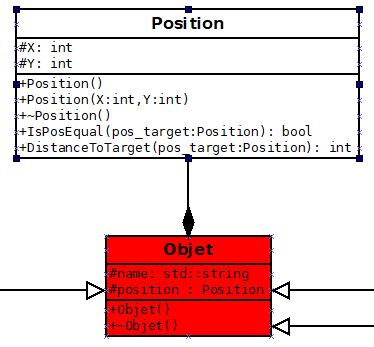
\includegraphics[width=0.5\textwidth]{pics/final_state/classe_Objet1.PNG}
\caption[Bloc "Objet"]{\label{figure_simple}Bloc "Objet"}
\end{figure}

On peut distinguer les classes filles qui héritent directement de la classe “Objet” :

\begin{itemize}
    \item La classe "Ship" est la classe qui contient toutes les informations des vaisseaux. Chaque vaisseau est associé des statistiques.  On associe
également par relation de composition une structure “ShipStats” décrivant
le type de vaisseau, ainsi qu’une énumération “Ship-TypeID” exposant sa
classe de vaisseau.
\begin{figure}[!h]
\centering
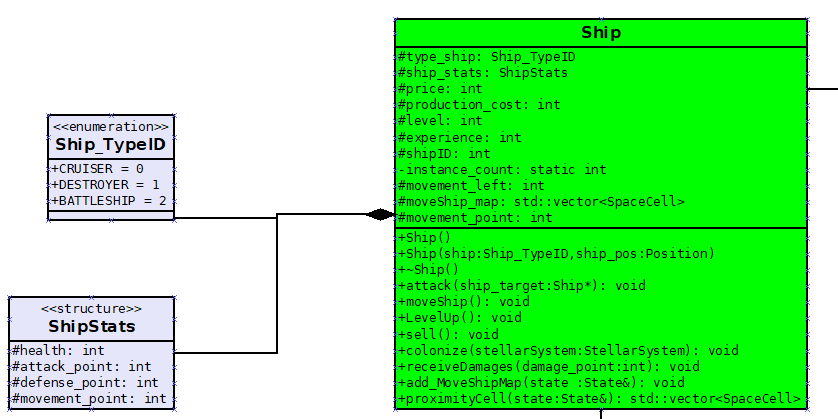
\includegraphics[width=0.8\textwidth]{pics/final_state/classe_vaisseau1.PNG}
\caption[Bloc "Ship"]{\label{figure_simple}Bloc "Ship"}
\end{figure}

\item La classe "StellarSytem" est la classe qui contient toutes les informations sur les systèmes stellaires. On retrouve par exemple la liste des buildings, le type d'environnement du StellarSystem, son statut de colonisation ainsi que sa taille. \\

\begin{figure}[!h]
\centering
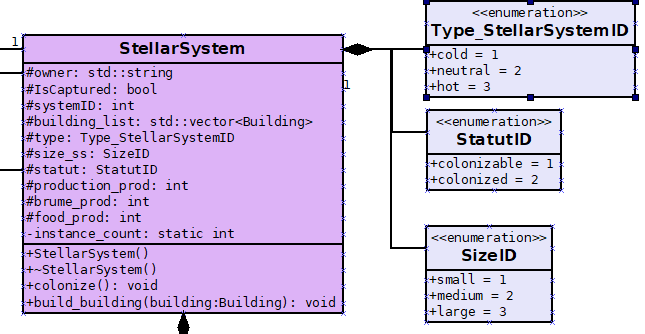
\includegraphics[width=0.6\textwidth]{pics/final_state/classe_StellarSystem.PNG}
\caption[Bloc "StellarSytem"]{\label{figure_simple}Bloc "StellarSytem"}
\end{figure}

Elle est associée à deux sous classes "Building" et "Planet".\\

\item La classe "Building" est la classe qui contient toutes les informations sur les Buildings. Chaque "Building" est associée à une "Ressources" en particulier, celle que le bâtiment va produire. De plus dans la classe on retrouve le prix dans chaque ressource permettant la construction du building ainsi que sa production par tour. La méthode "upgradeBuilding" permet elle d'augmenter la production du building. \\

\begin{figure}[!h]
\centering
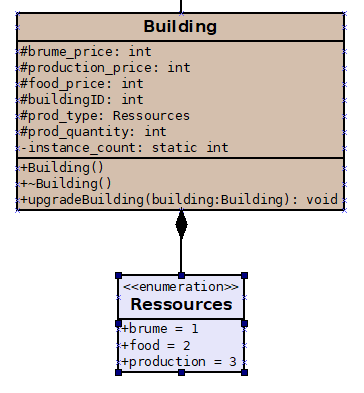
\includegraphics[width=0.6\textwidth]{pics/final_state/classe_batiment1.PNG}
\caption[Bloc "Building"]{\label{figure_simple}Bloc "Building"}
\end{figure}

\item La classe "Planet" a elle été mise de côté pour simplifier le nomnbre d'objets dans notre jeu,  nous avons donc transférer certains de ses attributs et méthodes dans la classe "StellarSystem". \\ \\ \\

\begin{figure}[!h]
\centering
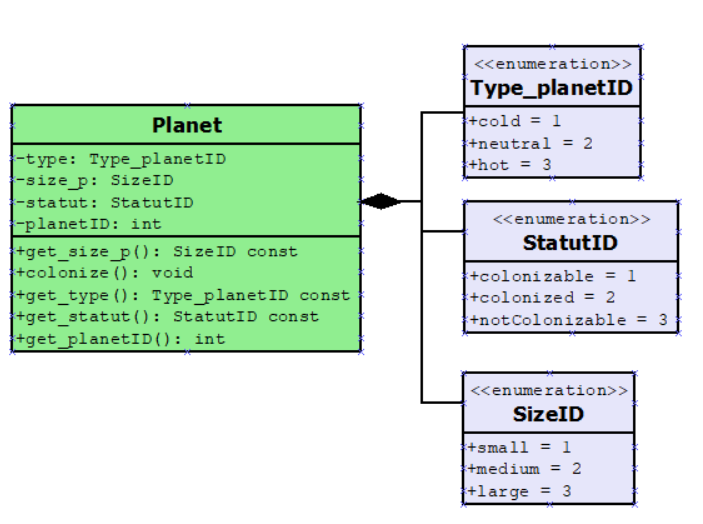
\includegraphics[width=0.6\textwidth]{pics/classe_planet.PNG}
\caption[Bloc "Planet"]{\label{figure_simple}Bloc "Planet"}
\end{figure}

\item La classe "SpaceCell" défini chacune des cases de notre jeu, elle permet dans la classe "State" de définir une map. \\

\begin{figure}[!h]
\centering
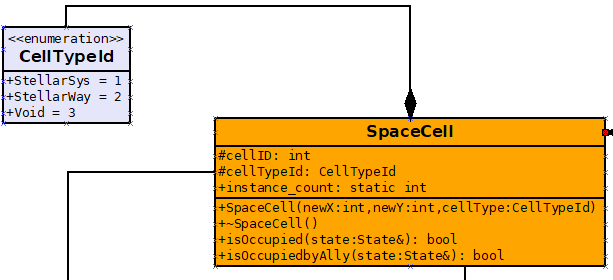
\includegraphics[width=0.6\textwidth]{pics/final_state/classe_SpaceCell1.PNG}
\caption[Bloc "SpaceCell"]{\label{figure_simple}Bloc "SpaceCell"}
\end{figure}

\item La classe " Player" est la classe qui va centraliser l'ensemble des informations concernant le joueur. Le joueur se voit associé des vaisseaux, des systèmes stellaires, des bâtiments,.. Il possède aussi diffèrent type de ressources, " Ressource".  \\ \\
\\

\begin{figure}[!h]
\centering
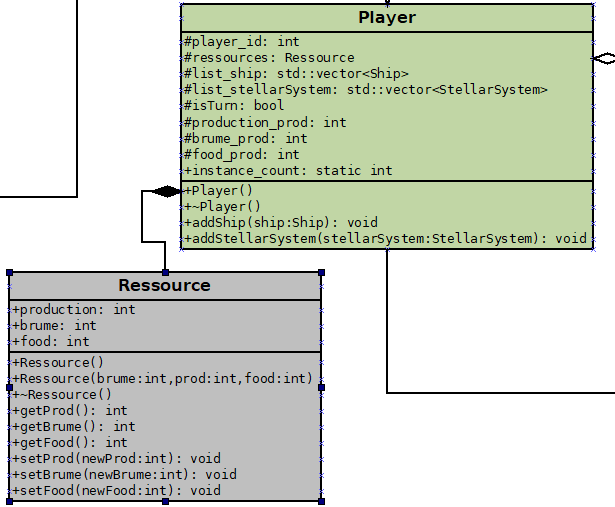
\includegraphics[width=0.8\textwidth]{pics/final_state/classe_player1.PNG}
\caption[Bloc "Player"]{\label{figure_simple}Bloc "Player"}
\end{figure}

\item La classe "State"  contient les classes "Player" et "SpaceCell". Cette classe donne l'état complet du jeu, la plupart des informations sont dans la classe "Player" et donc dans "Player a" et "Player b". \\


\begin{figure}[!h]
\centering
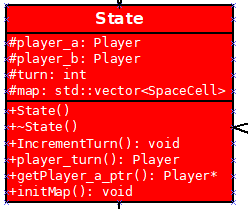
\includegraphics[width=0.3\textwidth]{pics/final_state/classe_state1.PNG}
\caption[Bloc "State"]{\label{figure_simple}Bloc "State"}
\end{figure}

\item Finalement, on peut voir notre diagramme d'états entier sur la figure suivante : 

\begin{figure}[!h]
\begin{center}
\rotatebox{270}{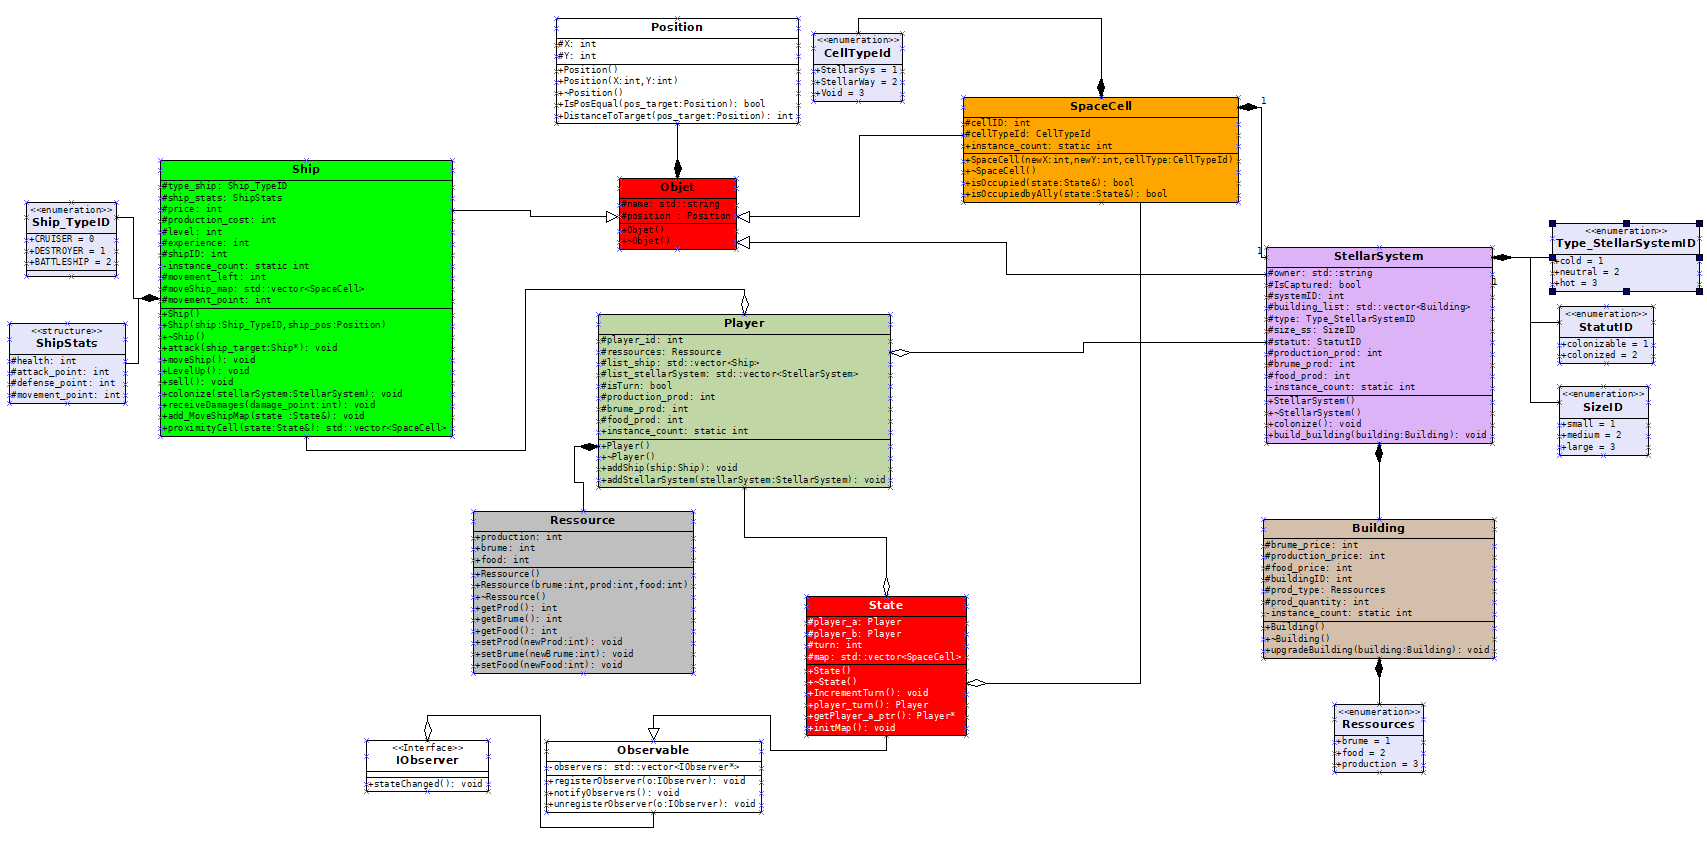
\includegraphics[width=1.4\textwidth]{pics/final_state/ensemble_classe1.PNG}}
\end{center}
\caption[State diagram]{\label{figure_simple}State diagram}
\end{figure}
\end{itemize}

\chapter[Description et Conception du Rendu]{Description et Conception du Rendu}
\chaptermark{Description et Conception du Rendu}
\section{Description des états}

\begin{figure}[!h]
\centering
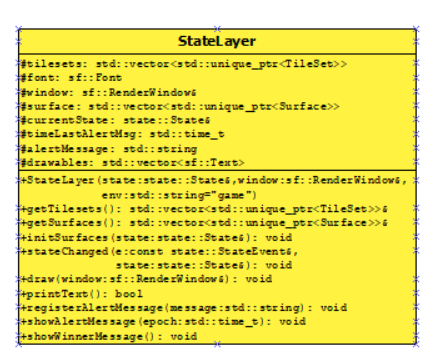
\includegraphics[width=1\textwidth]{pics/statelayer.PNG}
\caption[Bloc "statelayer"]{\label{figure_simple}Bloc "statelayer"}
\end{figure}

\begin{figure}[!h]
\centering
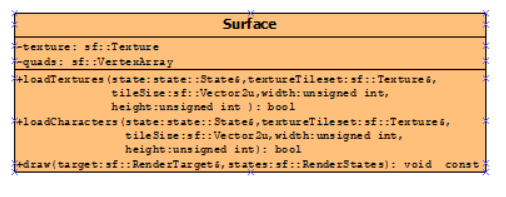
\includegraphics[width=1\textwidth]{pics/surface.PNG}
\caption[Bloc "surface"]{\label{figure_simple}Bloc "surface"}
\end{figure}

\begin{figure}[!h]
\centering
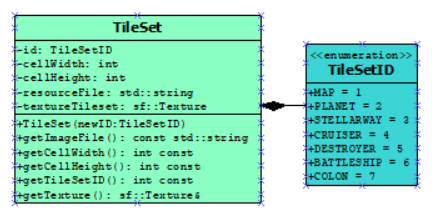
\includegraphics[width=1\textwidth]{pics/tileset.PNG}
\caption[Bloc "tileset"]{\label{figure_simple}Bloc "tileset"}
\end{figure}

\begin{figure}[!h]
\centering
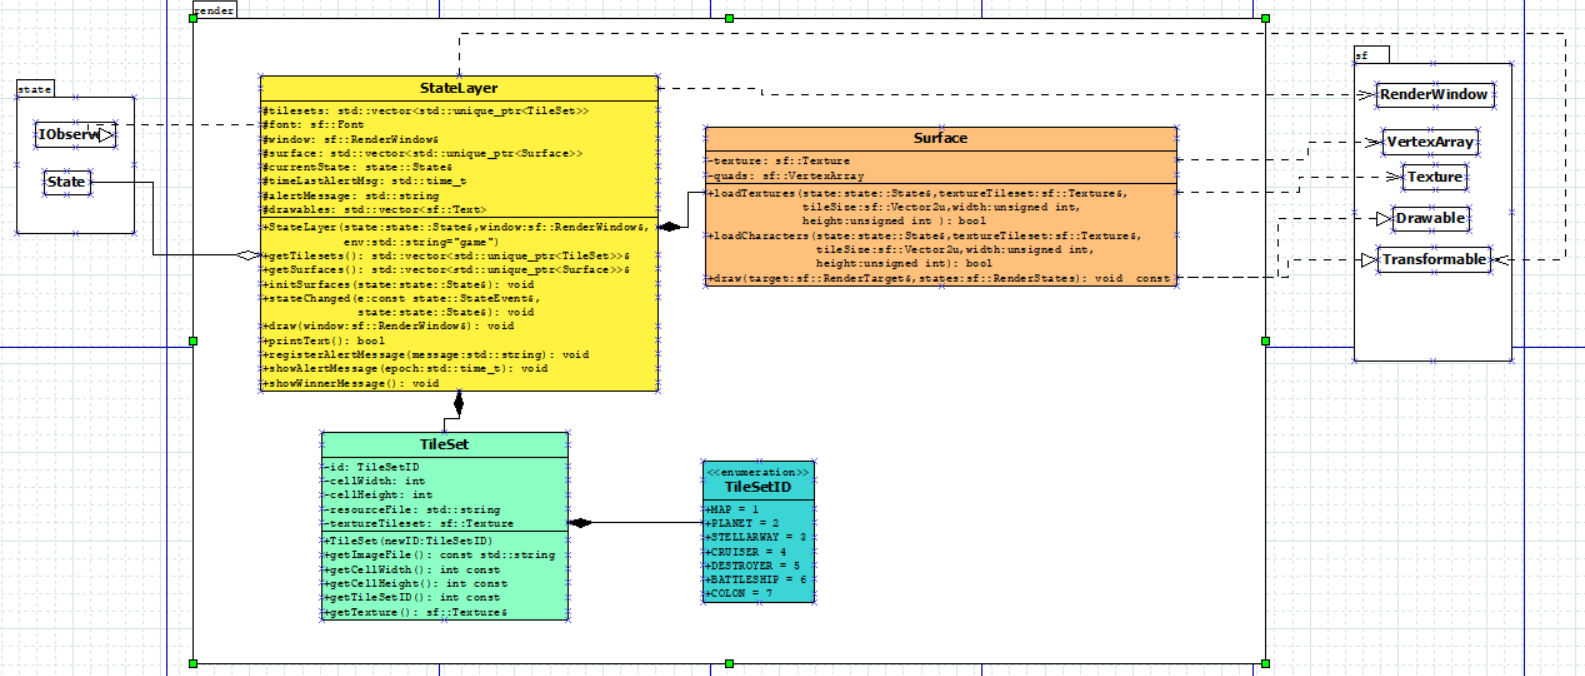
\includegraphics[width=1\textwidth]{pics/render.PNG}
\caption[Bloc "render"]{\label{figure_simple}Bloc "render"}
\end{figure}

\begin{figure}[!h]
\centering
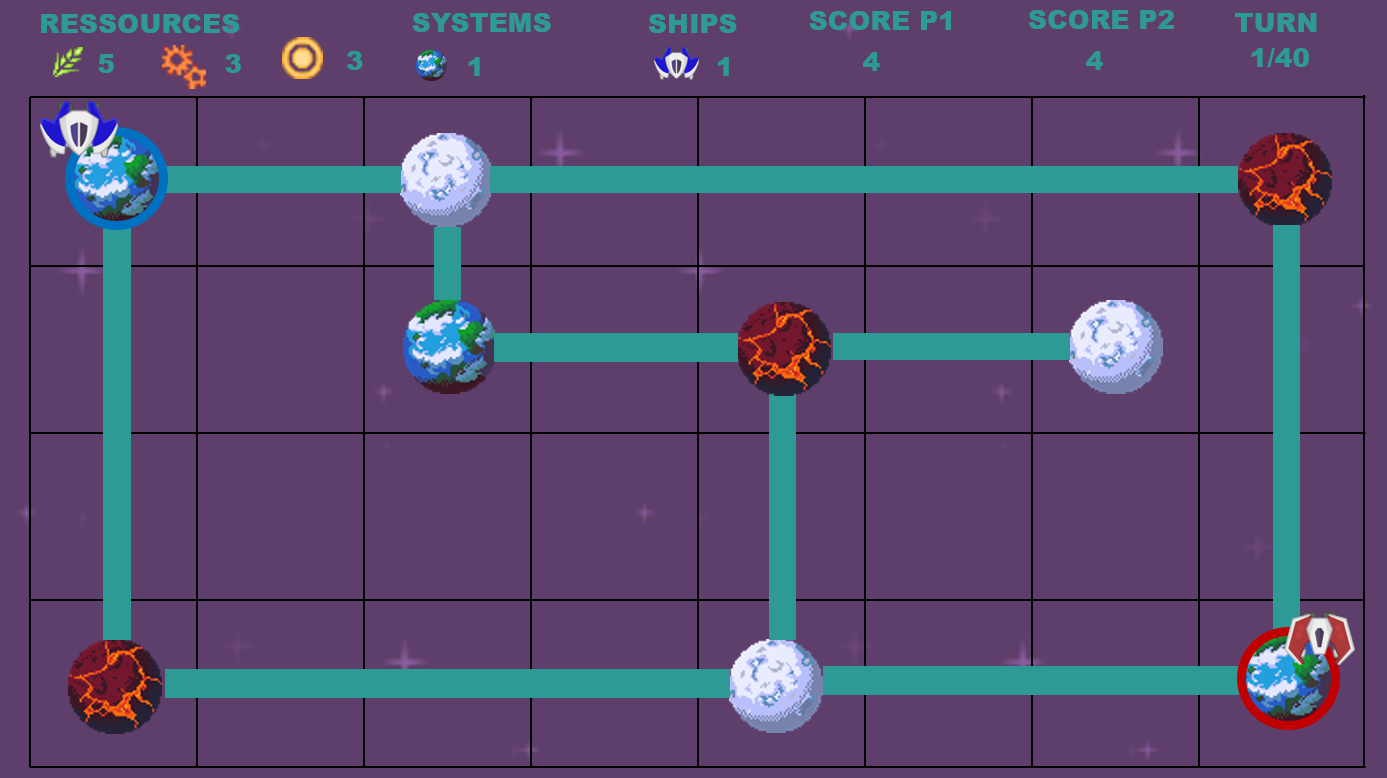
\includegraphics[width=1\textwidth]{pics/rendu.PNG}
\caption[Exemple d'affichage]{\label{figure_simple}Exemple d'affichage}
\end{figure}



\chapter[Moteur de Jeu]{Moteur de Jeu}
\chaptermark{Moteur de Jeu}
\section{Actions utilisateur} 

Le joueur va devoir allier un grand nombre d'actions par tour. Pour cela il aura la possibilité de choisir parmi les commandes suivantes : \\ \\
- Sélectionner un vaisseau :  \textbf{SelectShipCommand}. \\
- Déplacer un vaisseau :  \textbf{MoveCommand}.\\
- Attaquer un vaisseau ennemi :  \textbf{AttackCommand}. \\
- Coloniser une planète à l'aide d'un vaisseau :  \textbf{ColonizeCommand}. \\
- Construire un bâtiment ou un vaisseau :  \textbf{BuildBuildingCommand} ou  \textbf{BuildShipCommand}. \\
- Terminer son tour : \textbf{FinishTurnCommand}. \\ \\
Pour effectuer les commandes concernant un vaisseau, le joueur devra préalablement sélectionner le vaisseau avec lequel il veut effectuer une action.

\section{Action automatique}

A chaque fin de tour, le jeu va venir appeler la fonction "CheckWinnerCommand" afin de déterminer si oui ou non la partie doit s'arrêter.

\section{Description logicielle}

L'ensemble des commandes contiennent un constructeur permettant de leur attribuer leur commandID. \\
De plus, elles possèdent toutes la méthode "serialize" permettant de mettre sous format Json l'ensemble des informations utiles concernant la commande.

\subsection{Command}

Cette classe permet de décrire l'ensemble des commandes. \\
Elle contient 2 attributs, l'un pour préciser lequel des joueurs effectue les commandes, l'autre pour préciser l'ID de la commande, c'est à dire la commande à effectuer. La méthode "execute" est elle définie par la méthode du même nom appartenant à la classe fille dont il est question.\\
L'ensemble des commandes héritent de cette classe.\\

\begin{figure}[!h]
\centering
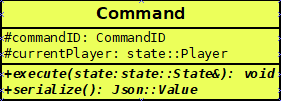
\includegraphics[width=0.5\textwidth]{pics/engine_pics/command.PNG}
\caption[Bloc "Command"]{\label{figure_simple}Bloc "Command"}
\end{figure}

\subsection{SelectShipCommand}

Cette commande permet de sélectionner le vaisseau "target" sur lequel on veut effectuer des actions.
La méthode execute vient vérifier si le vaisseau ciblé appartient bien au joueur effectuant la commande. Si c'est le cas elle permet alors l'affichage des différentes commandes permettant les actions du vaisseau.
\\
\begin{figure}[!h]
\centering
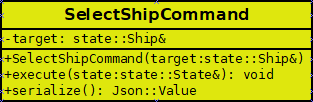
\includegraphics[width=0.5\textwidth]{pics/engine_pics/SelectShipCommand.PNG}
\caption[Bloc "SelectShipCommand"]{\label{figure_simple}Bloc "SelectShipCommand"}
\end{figure}

\subsection{MoveCommand}

Cette commande possède 2 attributs lui permettant de définir le vaisseau "ShipTarget" à déplacer et la position "PositionTarget" sur laquelle il souhaite le déplacer. \\
La méthode "execute" vient regarder si le déplacement est possible : \\
- aucun vaisseau allié est sur la position indiqué, \\
- la position ciblée est bien une SpaceCell de type "StellarSyst" ou "StellarWay", \\
- et enfin, si la position ciblée est bien dans la portée de déplacement du vaisseau. \\
Elle mets ensuite à jour la position du vaisseau ainsi que ses points de mouvement restants.
\\
\begin{figure}[!h]
\centering
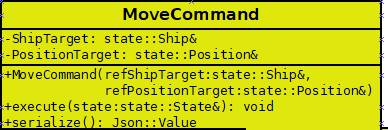
\includegraphics[width=0.5\textwidth]{pics/engine_pics/MoveCommand.PNG}
\caption[Bloc "MoveCommand"]{\label{figure_simple}Bloc "MoveCommand"}
\end{figure}

\subsection{AttackCommand}

Cette commande possède 2 attributs définissant le vaisseau "attacker" et le vaisseau "target". \\
La méthode "execute" vient vérifier que l'action d'attaque est bien possible c'est à dire que les 2 vaisseaux se trouvent bien sur la même position. Elle compare ensuite les types des vaisseaux pour actualiser l'état de chacun d'entre eux (destruction ou perte de point de vie).
\\
\begin{figure}[!h]
\centering
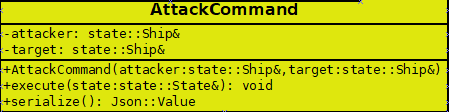
\includegraphics[width=0.5\textwidth]{pics/engine_pics/AttackCommand.PNG}
\caption[Bloc "AttackCommand"]{\label{figure_simple}Bloc "AttackCommand"}
\end{figure}

\subsection{BuildBuildingCommand et BuildShipCommand}

Ces 2 commandes ont un fonctionnement similaire. Elles permettent la construction d'un building ou d'un ship sur le système stellaire "StellarTarget". \\ La méthode "execute" vérifie si la construction est possible : \\
- StellarTarget est bien un système stellaire appartenant au joueur,\\
- et le joueur possède le nombre de ressources nécessaire à la construction. \\
La méthode ajoute donc l'objet construit à la liste de ship ou de building du joueur et actualise la production du système dans le cas de la construction du building.
\\
\begin{figure}[!h]
\centering
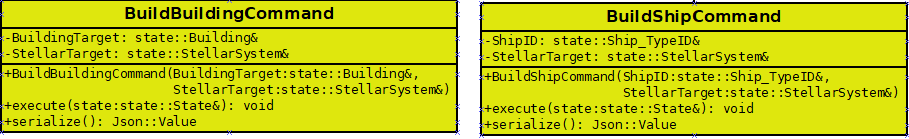
\includegraphics[width=1\textwidth]{pics/engine_pics/BuildsCommand.PNG}
\caption[Bloc "BuildBuildingCommand et BuildShipCommand"]{\label{figure_simple}Bloc "BuildBuildingCommand et BuildShipCommand"}
\end{figure}

\subsection{FinishTurnCommand}

Cette commande permet au joueur de mettre fin à son tour, d'incrémenter le nombre de tour dans la classe State pour permettre à l'autre joueur de jouer. \\
La méthode "execute" vérifie bien que c'est le joueur qui joue le tour qui effectue cette commande.

\begin{figure}[!h]
\centering
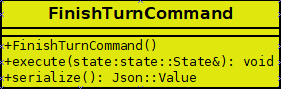
\includegraphics[width=0.5\textwidth]{pics/engine_pics/FinishTurnCommand.PNG}
\caption[Bloc "FinishTurnCommand"]{\label{figure_simple}Bloc "FinishTurnCommand"}
\end{figure}

\subsection{CheckWinnerCommand}

Cette commande permet à chaque fin de tour de vérifier si il y a un vainqueur. \\ 
La méthode "execute" vérifie que chacun des joueurs possèdent au moins 1 système stellaire ou 1 vaisseau. Dans le cas contraire il déclare vainqueur (victoire militaire) le joueur ayant toujours au moins un de ces objets. Si aucun joueur n'est gagnant à la fin d'un nombre de tour prédéfini (40 par exemple), alors il vient comparer les scores de chacun des joueurs pour déclarer gagnant le joueur ayant le plus de score.

\begin{figure}[!h]
\centering
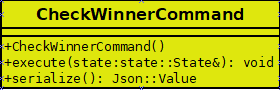
\includegraphics[width=0.5\textwidth]{pics/engine_pics/CheckWinnerCommand.PNG}
\caption[Bloc "CheckWinnerCommand"]{\label{figure_simple}Bloc "CheckWinnerCommand"}
\end{figure}

\chapter[Intelligence Artificielle]{Intelligence Artificielle}
\chaptermark{Intelligence Artificielle}
\section{Intelligence Artificielle Aléatoire}

Notre Intelligence Artificielle va devoir s'expandre et se développer, nous allons donc dans un premier temps effectuer aléatoirement les actions liées aux vaisseaux puis celles liées aux systèmes.
Dans un premier temps, la stratégie pour les vaisseaux suit simplement le diagramme suivant :

\begin{figure}[!h]
\centering
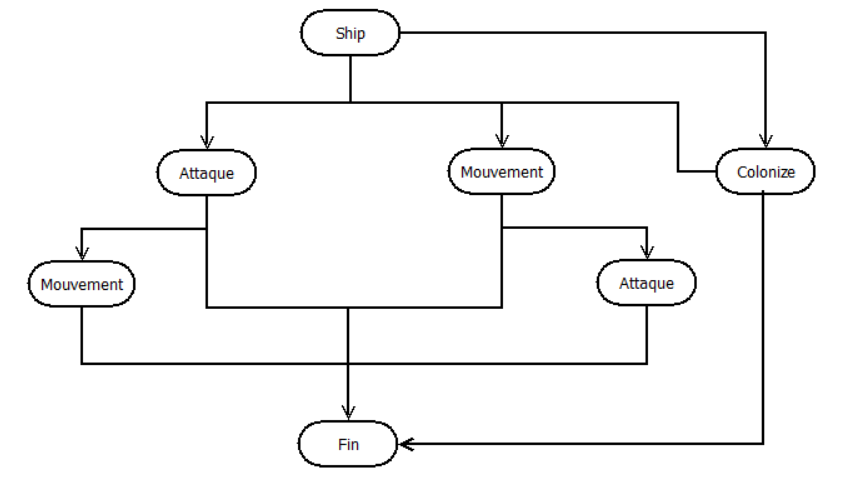
\includegraphics[width=1\textwidth]{pics/IA_random.PNG}
\caption[Stratégie d'expansion]{\label{figure_simple}Stratégie d'expansion}
\end{figure}



\begin{itemize}
\item L'IA va sélectionner un vaisseau,
\item Elle va ensuite choisir aléatoirement une action parmi les 3 disponibles sachant que l'action de coloniser à une probabilité plus élevé que les deux autres,
\item Selon l'action qu'elle a effectué elle pourra déplacer ou attaquer, si elle choisit la commande de colonisation et qu'elle est possible le vaisseau est alors détruit sinon on teste les commandes d'attaque et de déplacement,
\item Finalement si il reste des vaisseaux disponible, on recommence le même paterne 
\end{itemize}

Dans un second temps, la stratégie de développement des systèmes et la suivante : 

\begin{figure}[!h]
\centering
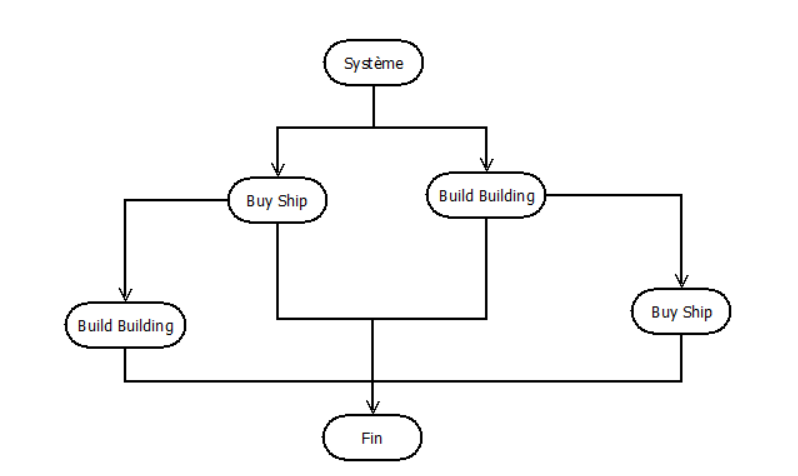
\includegraphics[width=1\textwidth]{pics/IA_random2.PNG}
\caption[Stratégie de développement]{\label{figure_simple}Stratégie de développement}
\end{figure}

\begin{itemize}
\item L'IA va sélectionner un système,
\item Elle va alors choisir aléatoirement entre construire un bâtiment ou acheter un vaisseau,
\item Si une commande est effectuée, on passe à un autre système disponible sinon on test l'autre commande,
\item Finalement on passe à un autre système disponible
\end{itemize}

\section{Intelligence Artificielle Heuristique}

Nous allons maintenant voir l'IA heuristique qui va prendre de meilleurs décisions que l'IA aléatoire. Nous avons implémenter des poids sur certaines commandes en fonction de sa situation actuelle et celle de l'adversaire.
Pour la partie expansion. Un vaisseau n'attaquera plus les vaisseaux qui ont un avantages sur lui, il favorisera la colonisation de nouveaux systèmes
Pour la partie développement, cela dépendra principalement de la flotte de l'adversaire :\\

\begin{itemize}
    \item Si l'IA possède une flotte de vaisseaux qui ont l'avantage sur celle de l'adversaire, l'IA va alors préférer la construction de nouveau bâtiment pour augmenter sa production de ressources. 
    \item Si la flotte de l'IA est plus faible que celle de l'adversaire, l'IA va alors favoriser l'achat de vaisseaux qui contre la flotte actuelle de l'adversaire.
\end{itemize}


%%%% Bibliography before appendices
%%%% After the initial round, you need to fix it by hand depending on where you generate your .bib file from
%%%% Mendeley often messes with italics and accents for instance


\end{document}
